%!TEX program = xelatex
\documentclass[a4paper,12pt]{report}
\usepackage[left=3cm, right=2.5cm, top=2.3cm, bottom=3.5cm]{geometry}
\usepackage{amsmath}
\usepackage{amsfonts}
\usepackage{amssymb}
\usepackage{algpseudocode}
\usepackage{algorithm}
\usepackage{graphicx}
% \usepackage{subfigure} % this package will cause error for subfigure, use caption & subcaption instead
\usepackage{caption}
\usepackage{subcaption}
\usepackage{enumerate}         
\usepackage{titlesec}
\usepackage{url}
\usepackage{color}
\usepackage{tabu}
\usepackage{makecell}
\usepackage[table]{xcolor}
\usepackage[T1]{fontenc}
\usepackage{enumitem}
\usepackage{cite}
\usepackage{amsmath}
\DeclareMathOperator*{\argmin}{argmin} % thin space, limits underneath in displays
\DeclareMathOperator*{\argmax}{argmax} % thin space, limits underneath in displays

\usepackage[redeflists]{IEEEtrantools}

\newcommand{\tabincell}[2]{\begin{tabular}{@{}#1@{}}#2\end{tabular}}
\renewcommand{\baselinestretch}{1.5}
\parindent=0pt
\titleformat{\chapter}[block]{\LARGE\bfseries}{\chaptertitlename\ \thechapter}{1em}{\LARGE}
\graphicspath{ {./images/} }

\title{A Comparative Study on Recommendation Systems for Multimedia \\}
\author{Student: Wei-Cheng Lin \\
Advisor: Prof. Sok-Ian Sou\\
\\
Department of Electrical Engineering  \\
National Cheng Kung University \\
Thesis for Master of Science Degree \\
}
\date{July, 2022}

\allowdisplaybreaks[1] 

\begin{document}
\bstctlcite{IEEEexample:BSTcontrol}

\maketitle

\begin{titlepage}
    \begin{center}
        {\bf\large A Comparative Study on Recommendation Systems for Multimedia}\\
        {Postgraduate: Wei-Cheng Lin \hspace{8mm} Advisor: Prof. Sok-Ian Sou}\\
        {Department of Electrical Engineering}\\
        {National Cheng Kung University}\\
    \end{center}

    \paragraph{}
    \begin{center}
        {\bf Abstract}\\
    \end{center}
    \paragraph{}
    With the rapid growth of streaming services and data on the Internet, people are faced with more choices, and it becomes harder for people to find their preferred items. To this end, many recommender systems are proposed and become practical tools to list potential items users want to buy. Many studies have shown that the recommender system is helpful for music and movie recommendations. However, most of the previous studies and related datasets focus on the recommendation performance of western music; which lacks the performance of making recommendations when it comes to Chinese music. This paper provides a study and analysis of several recommendation algorithms. We also implemented the recommendation algorithms on two real-world multimedia datasets: MovieLens and MuTube; the latter dataset comprises Taiwanese users' listening histories and Chinese music. Experimental results represent that contextual information and content-based filtering is a suitable way to consider the trade-off between evaluation metrics such as Top-N accuracy, diversity, novelty, and response time compared with the other existing approaches on both datasets.\\
 
    \textbf{Keywords:} {recommender system, collaborative filtering, hybrid filtering, SVD, multimedia, music, movie, contextual information, novelty, diversity}
\end{titlepage}

\pagenumbering{roman}
\setcounter{page}{4}
\addcontentsline{toc}{section}{Contents}
\tableofcontents \newpage
\addcontentsline{toc}{section}{List of Figures}
\listoffigures \newpage
\addcontentsline{toc}{section}{List of Tables}
\listoftables \newpage
\pagenumbering{roman}

\setcounter{page}{1}
\pagenumbering{arabic}

%*---------------------Introduction----------------------------------
\chapter{Introduction}

\paragraph{}
Nowadays, online services have become part of our daily life. Many people's daily routines include watching videos and movies and listening to music on streaming platforms in their spare time. However, the convenience of online streaming services leads to a massive amount of information and data on the Internet, making it difficult for users to discover desirable items and make decisions efficiently; such a problem is called information overload. Recommender systems were introduced to filter relevant content and overcome the problem of information overload. They became a necessary technique to help people efficiently find their preferred items.
%---
\paragraph{}
The recommender systems can be categorized into two types on the basis of recommendation approaches, which are called Collaborative Filtering\cite{sarwar2001item,linden2003amazon,bennett2007netflix,breese2013empirical,Reddy2014music,Barathy2020Matrix} and Content-based Filtering\cite{basu1998recommendation,van2000using,pazzani2007content,cantador2010content,Singla2020flex}. For Collaborative Filtering, it finds the correlation among users based on their historical behavior, defines similar users, and then produces recommendations according to similar users' preferred items. On the other hand, Content-based Filtering explores items' attributes by feature extraction and calculates the similarity of items. The users' profiles will be built by observing their past behavior, and Content-based filtering will recommend items that are similar to the ones that user has highly rated before without considering other users' opinions. Both approaches have their drawbacks and limitations. Collaborative filtering requires many interactions between users and items to make recommendations. When the user-item matrix is sparse,  the quality of recommendations will suffer from the problem of data sparsity and become less efficient. Content-based filtering requires domain knowledge and metadata of users and items which might not be available and easy to collect. Besides, Content-based filtering suffers from the novelty problem, which implies that the recommended items are always similar to the ones users liked in the past. The recommendation becomes a lack of novelty then.
%---
\paragraph{}
Many studies on recommender systems for multimedia such as movies and music have been conducted. Also, many public multimedia datasets, such as Spotify\cite{spotify2018} and Last.fm\cite{vigliensoni17music,Bertin-Mahieux2011}, are widely used in the research of recommender systems. However, the datasets used in most previous studies only focus on Western music. We cannot evaluate the performance of recommendation approaches when it comes to the datasets that consists of Chinese songs. In this work, we use two datasets to study recommender systems. The MuTube\cite{MuTube2020ICS} dataset for music recommendation while the famous MovieLens\cite{harper2015movielens} dataset for movie recommendation. The former dataset mostly comprises Taiwanese users' listening behavior and Chinese music, and the latter dataset is published by GroupLens research group and comprised of users' ratings on movies. We perform several recommendation approaches on the datasets mentioned above and evaluate the recommendation quality. Since accuracy is not enough to thoroughly measure the quality recommendation approach, for example, the recommended items are always the most popular can lead to high accuracy. At the same time, the users rarely get pleasantly surprised. As a result, we also evaluate the diversity and novelty of recommendation approaches in this paper and find the trade-off between accuracy, diversity, novelty, and response time.
%---
\paragraph{}
The remainder of the paper is organized as follows: Chapter 2 reviews the related work of the recommender system. The detailed information on datasets is introduced in Chapter 3. In Chapter 4, we explain our proposed framework for predicting users' preferences. Experimental setup and analyses of recommendation approaches will be presented in Chapter 5, and Chapter 6 provides the conclusion and future works.

%*---------------------Introduction----------------------------------
%*---------------------Related Work----------------------------------
\chapter{Related Work}
\paragraph{}
Recommender systems are mostly based on two categories: Collaborative Filtering (CF) and Content-based Filtering (CBF). Also, several hybrid recommendation approaches have been proposed by merging the two types of recommender systems to overcome the limitations of CF and CBF individually, which is called Hybrid Filtering. In this chapter, a review of past studies is presented by categories.

\section{Collaborative Filtering}
\paragraph{}
Collaborative Filtering (CF) approaches build the system based on the interactions between users and items, such interactions include ratings, listening counts, and purchase histories; which becomes helpful in constructing the rating matrix between users and items. CF approaches will find users with similar tastes for a particular user, and then create a ranked list of recommendations by considering what similar users like instead of features of the items. Singular Value Decomposition (SVD) has become a popular CF approach since Netflix prize\cite{bennett2007netflix}; it reduces the space dimension and gives the best low-rank approximation by selecting k-largest singular value from the factorization of the original user-item matrix, which implies that noise data will be removed and the latent relationship between users and items can be found. 

\section{Content-based Filtering}
\paragraph{}
Content-based filtering (CBF) approaches create a profile for each item or user based on the features (e.g., item tags, genres, age of users, or gender) which might be already provided in the dataset. CBF uses the content analyzer to extract the characteristic of users' favorite items based on their past behavior, then the system will find the Top-N items with the most similar content to the particular user's profile and create a ranked list of recommendations.

\section{Hybrid Filtering}
\paragraph{}
Both CF and CBF have their pros and cons, hence, the idea of Hybrid Filtering is to merge different recommendation approaches (mostly CF and CBF) to achieve better recommendation performance and overcome the different limitations of each recommendation approach. Osmanlı, $et\ al.$\cite{osmanli2011using} utilizes tags of movies as additional information. The original user-item matrix is extended with tagging information before conducting SVD such that the system can provide better recommendations by inspecting the latent relationship among users, items, and tags.
%*---------------------Related Work----------------------------------

%*---------------------Datasets--------------------------------------
\chapter{Datasets}
\paragraph{}
The following chapters evaluate the performance over two real-world datasets: HetRec-2011-movielens-2k dataset and MuTube dataset. Before introducing the evaluation metrics and the compared recommendation approaches, we want to first give an insight into both datasets in this chapter. 
%---
\section{MovieLens Dataset}
\paragraph{}
For movie recommendations, the HetRec-2011-movielens-2k dataset is an extension of the MovieLens-10M dataset and published by GroupLens. It contains about 860,000 rating data of 10197 different movies created by 2113 users; movies are rated with scores 1-5. Aside from rating data, the tagging information is also included in the dataset. We can find the tag assignments of the movies provided by each user in the dataset. 
\section{MuTube Dataset}
\paragraph{}
Many previous studies on recommendation systems use Last.fm as the dataset to evaluate the performance of recommendation algorithms. We also want to know the effectiveness of different recommendation algorithms when the tracks in the dataset are mostly Chinese music, hence, the MuTube dataset will be used for music recommendations in this study. Here, we would like to briefly describe the MuTube dataset and explain how we collect YouTube usage data and create this dataset.

\subsection{Data Collection}
\paragraph{}
MuTube is a Google Chrome extension based on JavaScript that collects YouTube usage data and other additional information. Once a user watches videos on YouTube, MuTube will record the listening behavior and collect the related data by using YouTube API. For video information, the metadata collected by MuTube is shown in Table.~\ref{tab:MuTube_video_metadata}. Also, MuTube will collect related information from the interactions between users and videos (i.e. listening behavior), such information is listed in Table.~\ref{tab:MuTube_listen_metadata}. The ``Listen Time", ``Like Status", and ``Count" are important attributes for evaluating whether the user enjoys this video.

\begin{table}[!htbp]
    \caption{The metadata of videos being collected in the MuTube dataset}
    \centering
    \begin{tabular}{|c|l|}
    \hline
    Attribute     & Description \\
    \hline
    Video ID & Unique ID that YouTube uses to identify different videos. \\
    \hline
    Video Title     & The video's title. \\
    \hline
    Duration & The length of the video in seconds. \\
    \hline
    Video Tags & \tabincell{l}{ A list of keywords, which is associated with current video. \\ The tags are provided by the video uploader. }\\
    \hline
    Channel Name & The channel name for the channel that uploads the video. \\
    \hline
    \end{tabular}
    \label{tab:MuTube_video_metadata}
\end{table}

\begin{table}[!htbp]
    \centering
    \caption{The related information of listening history}
    \begin{tabular}{|c|l|}
    \hline
    Attribute   &  Description\\
    \hline
    User ID     & Unique identifier for each different user. \\
    \hline
    Video ID & Unique ID that YouTube uses to identify different videos. \\
    \hline
    Listen Time & The view duration of a user watching the video in seconds. \\
    \hline
    Like Status & \tabincell{l}{A boolean value which represents whether the  user clicks\\ the like button.} \\
    \hline
    Count & View count of a single video by current user. \\
    \hline
    timestamp & The timestamps when the user plays a video (i.e. time logs). \\
    \hline
    \end{tabular}
    \label{tab:MuTube_listen_metadata}
\end{table}

\subsection{Data Cleaning}
\paragraph{}
The users of MuTube do not always only watch videos belong to ``music topic'' on YouTube, sometimes they watch different topics of videos such as gaming, sports, and lifestyle. However, the MuTube dataset is built to be a dataset for the research of music recommendation, the YouTube videos which are not music video must be removed as a result. There are 3 approach which are applied to filter out these items in MuTube. We will describe each approach individually.
\subsubsection{Video Duration}
\paragraph{}
The video duration of music videos on YouTube mostly ranges from 2 to 7 minutes. If the duration of a video is not in the range, it will be removed then.

\subsubsection{Categories of videos}
\paragraph{}
The category ID list of YouTube videos is shown in Table.~\ref{tab:MuTube_category_id}, and the owners of videos on YouTube can select the most appropriate category for their videos to get more views. Hence, we use the YouTube API to get the category ID of each video and filter out the one does not belong to the ``Music" category.
\begin{table}[!ht]
    \centering
    \caption{YouTube Video Category ID List}
    \begin{tabular}{|c|l|}
    \hline
    Category ID     &  Category Name \\
    \hline
    1     & Film \& Animation \\
    2     & Autos \& Vehicles \\
    10    & Music \\
    15    & Pets \& Animals \\
    17    & Sports \\
    \vdots     & \multicolumn{1}{c|}{\vdots} \\
    43    & Shows \\
    44    & Trailers \\
    \hline
    \end{tabular}
    \label{tab:MuTube_category_id}
\end{table}

\subsubsection{Keyword Dictionary}
In order to keep only music videos in the dataset, a keyword dictionary is created manually to remove the irrelevant videos based on their titles. For instance, the keyword dictionary contains keywords such as ``Covid-19", ``L'Occitane", and ``LOL Hightlight" and we believe that most of the videos with these keywords in their video titles are not music videos; therefore, the video will be removed if its title contains the keywords in the dictionary.
%---
\subsection{Word Segmentation for Video Title}
According to the tags provided by the owners of the videos, we can describe the style of the videos. However, not all video owners add tags when uploading videos, which means that not all videos have corresponding tags. Without tags, it becomes difficult to measure users' preferences. To this end, we segment the video titles and consider the results of word segmentation as additional tags; the original tag list of each different video will be extended with these additional tags, which increases the diversity of tags and can better describe the characteristic of each music video in MuTube.
%---
\subsection{MuTube Dataset Overview}
This dataset is comprised of 5,478 ratings from 25 users on 4,531 items, and tagging information is also available in MuTube. The users of MuTube are all from Taiwan and the tracks are mostly Chinese songs; and thus the performance of recommender systems for Chinese music can be evaluated. 
%---

\section{Statistics of two datasets}
\paragraph{}
The detailed information of the two datasets mentioned above is shown in Table~\ref{tab:datasets}. As we can see, the scope of MuTube dataset is relatively small compared to that of Movielens. In terms of the number of items on MuTube, it is similar to that on Movielens. However, the number of users on Movielens is about 80 times greater than that on MuTube. The top 10 tags for two datasets are shown in Table~\ref{tab:tags}. Most tags such as ``MayDay" and ``JayChou" can help users recognize and describe the characteristics of items, which means that tagging information can be utilized in the recommender system.
%---
\begin{table}[ht]
\caption{Statistics of datasets.}
\label{tab:datasets}
\begin{center}
\begin{tabular}[b]{l l l}
\hline
 & MovieLens & MuTube \\[0.3ex]
\hline
Type of content & movie & music \\[0.3ex]  
Users' ethnicity & American & Taiwanese \\[0.3ex]
Ratings  & 792,910 & 5,478 \\[0.3ex] 
Users & 2,113 & 25 \\[0.3ex]  
Items & 5,450 & 4,531 \\[0.3ex] 
Sparsity  & 93.10\%  & 95.16\% \\[0.3ex] 
Tags  & 4,417 & 18,723 \\[0.3ex] 
Avg. tags per item  & 8.28 & 11.59 \\
\hline
\end{tabular}
\end{center}
\end{table}

% Table
\begin{table}[ht]
\caption{Top tags for MovieLens and MuTube.}
\label{tab:tags}
\begin{center}
\begin{tabular}[b]{l l l }
\hline
rank & MovieLens & MuTube\\[0.3ex]
\hline
1 & tumey's dvds & MV \\[0.3ex]  
2 & classic & (MayDay) \\[0.3ex] 
3 & based on a book & (Jay Chou) \\[0.3ex] 
4 & nudity & (Ronghao Li) \\[0.3ex] 
5 & erland dvds & (Love Song) \\[0.3ex] 
6 & 70mm & (Ashin)  \\[0.3ex] 
7 & comedy & ONE OK ROCK  \\[0.3ex] 
8 & imdb top 250  & (JVR Music) \\[0.3ex] 
9 & action & (G.E.M.) \\[0.3ex] 
10& national film registry & (Eric Chou) \\
\hline
\end{tabular}
\end{center}
\end{table}

%*---------------------Proposed FrameWork---------------------------------
\chapter{Proposed Framework}
%*----------System Architecture------------
\section{Implicit Feedback Measurement}
\label{section:Implicit Feedback Measurment}
\paragraph{}
Recommender systems require various inputs to learn a user's preferences, and these inputs are generally explicit feedback and implicit feedback. Movie datasets such as Movielens\cite{harper2015movielens} enable users to express their opinions on movies directly. For example, a movie might receive a rating of 5 if the viewer enjoys watching it or a rating of 1 if the movie's content is irritating; such is referred to as explicit feedback and can be directly used as inputs in recommender systems. However, explicit feedback is not always available in a real-world scenario. In music datasets such as Last.fm\cite{Bertin-Mahieux2011,vigliensoni17music} and MuTube\cite{MuTube2020ICS}, These datasets contained only users' listening histories instead of direct ratings. Although it cannot use the listening histories as inputs for recommendation directly, we can still measure users' preferences based on the idea that the music a user listens to frequently should be the one the user prefers.
%---
\paragraph{}
To measure users' preferences in MuTube dataset, we first convert the listening histories into listening counts. The count$_{u,i}$ is defined as the times that user $u$ has listened to track $i$. The scale of total listening counts from each user is shown in Fig.~\ref{fig:total_listen_counts}. We can infer that users on the left-hand side are more active and tend to leave more logs than inactive users. Fig.~\ref{fig:act_user} represents an example of active user while Fig.~\ref{fig:inact_user} represents an example of inactive user. As shown in Fig.~\ref{fig:act_user},   if an active user listens to a track only three times, it shows that the user does not enjoy this track. However, for an inactive user, as shown in Fig.~\ref{fig:inact_user}, a low listening count does not always mean that the track does not appeal to the user. On the contrary, the listening count may be low because the user is less active. Thus, it could be risky if we use the listening counts information as ratings directly; it is necessary to normalize count$_{u,i}$ for each user in the dataset to achieve better measurement. We will implement two normalization strategies to convert listening counts into ratings individually and see which one can better deal with the skewed rating distribution.

% --- 分布圖
\begin{figure}
    \begin{center}
        \begin{subfigure}{.78\textwidth}
            \centering
            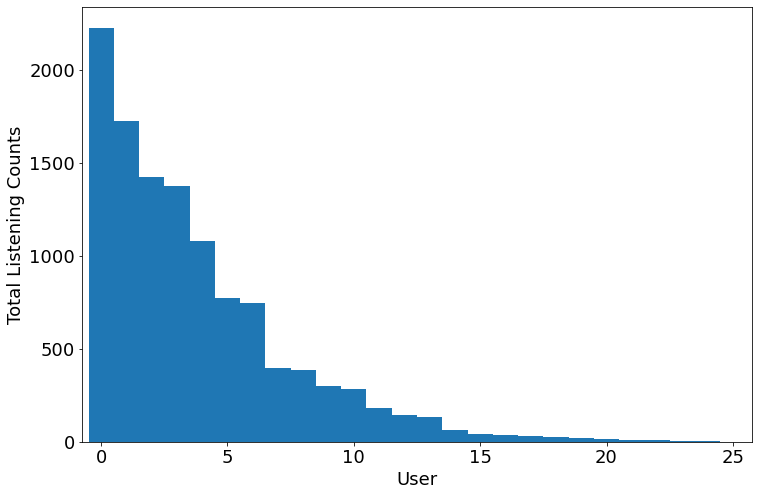
\includegraphics[width=1\linewidth]{./images/Total Listening Counts Bar}
            \caption{Total listening counts from each user in MuTube}
            \label{fig:total_listen_counts}
        \end{subfigure}
        \begin{subfigure}{.78\textwidth}
            \centering
            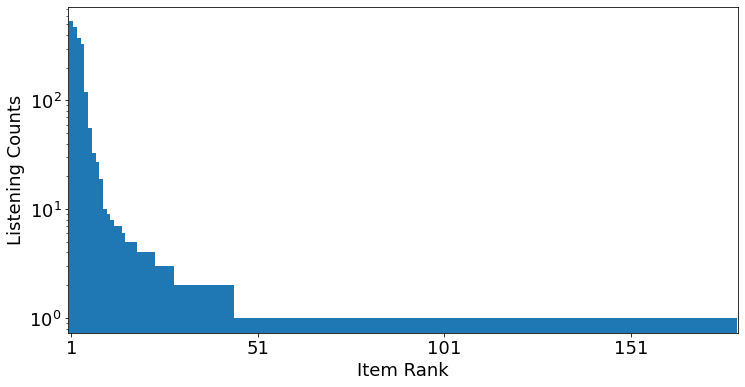
\includegraphics[width=1\linewidth]{./images/user_2}
            \caption{An active user}
            \label{fig:act_user}
        \end{subfigure}
        \begin{subfigure}{.78\textwidth}
            \centering
            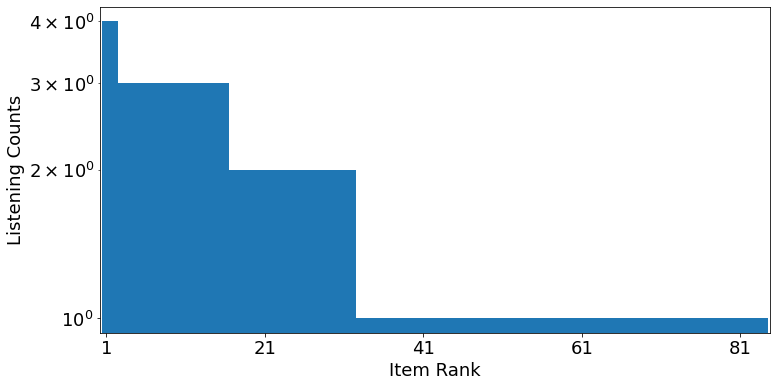
\includegraphics[width=1\linewidth]{./images/user_5}
            \caption{An inactive user}
            \label{fig:inact_user}
        \end{subfigure}
        \caption{Data visualization for users' listening behavior in MuTube}
        \label{fig:listen_behavior_MuTube}
    \end{center}
\end{figure}
% ---

% ---  Min-Max Normalization ----
\subsubsection{Min-max Normalization}
\paragraph{}
Min-max normalization is a common way to transform the range of features into the same scale. Since the scale of total listening count from each user is quite different, the listening count values must be shifted and rescaled so that the whole converted ratings can end up being in the same range, which is between 0 to 5. Eq.~\ref{eq:min-max} shows how min-max normalization is implemented. Count$_{u,min}$ is the listening count of user $u$'s least-listened track, which is set to 0 here; count$_{u,max}$ is the listening count of user $u$'s most-listened track.

\begin{equation}
    rating_{u,i} = 5\cdot\frac{count_{u,i}-count_{u,min}}{count_{u,max}-count_{u,min}}
    \label{eq:min-max}
\end{equation}



%\begin{figure}[t]
%    \centering
%    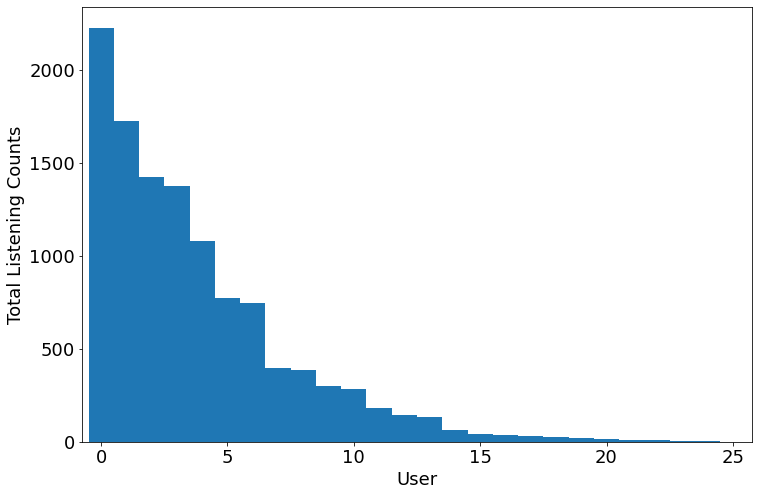
\includegraphics[width=\textwidth]{./images/Total Listening Counts Bar}
%    \caption{Total listening counts from each user in MuTube}
%    \label{fig:total_listen_counts}
%\end{figure}

%---

\subsubsection{Percentile Normalization}

\paragraph{}
Here, we borrow the concept from Pacula\cite{pacula2009matrix}, percentile normalization is utilized to convert the listening counts information into estimated ratings. First, we define $rank\_score$ in Eq.~\ref{eq:score}, where rank$_{u,i}$ and total$_{u}$ stand for the ranking of track $i$ listened by user $u$ and the number of tracks listened by user $u$ individually.

%--- Equation
\begin{equation}
    rank\_score_{u,i}= 5\cdot(1-\frac{rank_{u,i}}{total_u})
    \label{eq:score}
\end{equation}

% %---
% \begin{figure}[t!]
% \begin{center}
%     \begin{subfigure}{.96\textwidth}
%         \centering
%         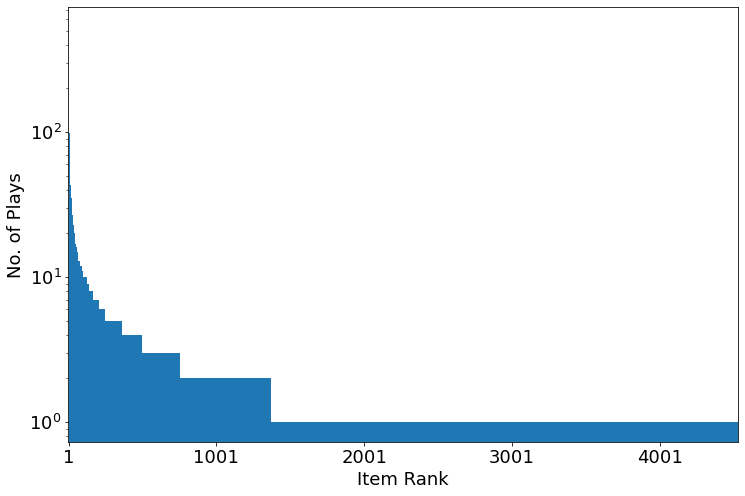
\includegraphics[width=1\linewidth]{./images/MuTube_longtail}
%         \caption{Distribution of each item's number of plays in MuTube}
%         \label{fig:longtail_MuTube}
%     \end{subfigure}
%     \begin{subfigure}{.96\textwidth}
%         \centering
%         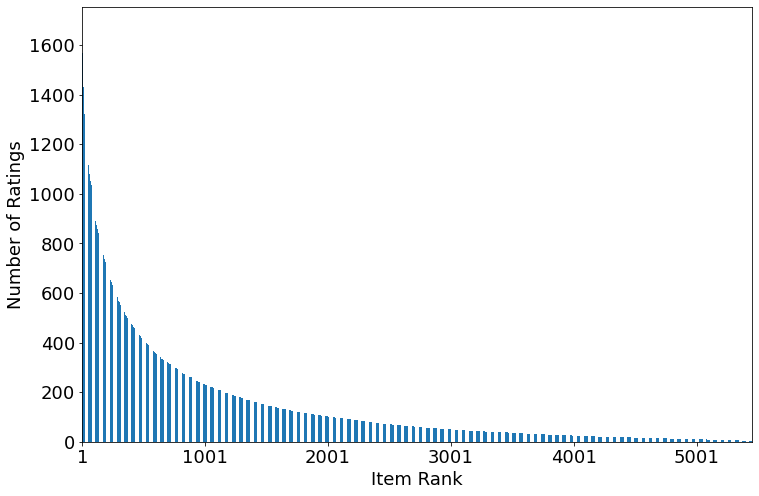
\includegraphics[width=1\linewidth]{./images/movielens_longtail}
%         \caption{Each item's number of ratings in Movielens}
%         \label{fig:longtail_ML}
%     \end{subfigure}
% \caption{Data Visualiztion for Long tail phenomenon in two datasets}
% \label{fig:long_tail}
% \end{center}
% \end{figure}

%---
\paragraph{}
Next, the rank scores are projected onto estimated ratings based on percentile normalization. The details of normalization rules are shown in Eq.\eqref{eq:rating}. In this way, we could use covert the data into five rating levels, and each level of ratings would contain 20\% of tracks that had been listened to by the user. For instance, the top 20\% most listened tracks will get an estimated rating of ``5", the subsequent 20\% ones will get ``4", and so on.
%=== Normalization === %
\begin{equation}
    \begin{aligned}
        r_{u}^5 &= \{i:5 > rank\_score_{u,i} \geq 4\}\\
        r_{u}^4 &= \{i:4 > rank\_score_{u,i} \geq 3\}\\
        r_{u}^3 &= \{i:3 > rank\_score_{u,i} \geq 2\}\\
        r_{u}^2 &= \{i:2 > rank\_score_{u,i} \geq 1\}\\
        r_{u}^1 &= \{i:1 > rank\_score_{u,i} \geq 0\}\\
    \end{aligned}
    \label{eq:rating}
\end{equation}

%---
\paragraph{}
The different scales of listening counts between users can be smoothed out by applying data normalization since the whole converted ratings are in the same range. In this way, each user's preferences can be well measured based on the listening counts information without considering whether the current user is active or not. We will compare each normalization strategy and show the distribution of estimated ratings in the next chapter.

%*-------------Tag Preference-------------
\section{Tag Preference Profile}
\paragraph{}
In Movielens and MuTube, tags are assigned to related items to describe their characteristics, which would help build profiles of users' tag preferences. Although there is no direct relationship between users and tags in both datasets, we can still measure users' tag preferences according to rating data. When a user rates an item, it can be regarded as implicitly giving ratings to corresponding tags. 
%---
%--- Tag relevance ---
\subsubsection{Tag relevance}
\paragraph{}
To construct a user-tag matrix, tag relevance must be measured first to know how important a particular tag is for describing the feature of the corresponding item. Tag weight stands for the relevance score on item-tag pair, which is already provided in the datasets; however, the maximum tag weight scores in different items vary in a wide range, so the normalization of tag weight is necessary. Again, we use percentile normalization to make tag weight scores categorized into five levels. The tags with the top 20\% most considerable tag weight for a particular item will get a converted tag relevance score of ``5" for this item; the subsequent ones will get ``4", and so on.

%--- Tag preference ----
\subsubsection{Tag preference}
\paragraph{}
In this step, the tag preference score of user $u$ to item $i$ is named as $pref_{u,t}$ and now can be derived from Eq.\eqref{eq:tag_pref}; where $I_u$ stands for the set of items that user $u$ has rated before and $Tag\_rel_{i,t}$ stands for the relevance score on item-tag pair which is acquired from tag weight provided in the datasets.

%--- Euqation ----
\begin{equation}
    pref_{u,t}= \sum_{i\in I_u} r_{u,i} \cdot Tag\_rel_{i,t}
    \label{eq:tag_pref}
\end{equation}
%---
\paragraph{}
After building a user-tag matrix for each user, it is evident that $pref_{u,t}$ differs on a large scale. Thus, before using tag preferences to generate a recommendation, we must perform normalization to make the tag preference scores range from 0 to 5, just like the user-item rating data does. Here, we use the min-max normalization strategy; since the minimum tag preference score must be 0, the normalization formula is shown in Eq.\eqref{eq:tag_norm}. Where $pref_{u,max}$ stands for the maximum tag preference score of user $u$. Using the tag preference score derived from normalization, we can finally build the profile of tag preferences for each user.
%---
\begin{equation}
    norm\_pref_{u,t} = 5 \cdot \frac{pref_{u,t}}{pref_{u,max}}
    \label{eq:tag_norm}
\end{equation}

%--------- Rating Prediction ---------
\section{Rating Prediction for Recommendation}
\paragraph{}
With the information above, tagging information can finally be incorporated into the recommendation algorithm. In the last step, the recommendation list for each user is generated by computing the predicted ratings for every user-item pair, which is shown as Eq.~\eqref{eq:pred_rating}.

\begin{equation}
    pred_{u,i} = \sum_{t\in i} norm\_pref_{u,t} \cdot Tag\_rel_{i,t}
    \label{eq:pred_rating}
\end{equation}

\chapter{Experimental Evaluation}
%*----------Experiment Setup---------
\section{Experiment Setup}
\paragraph{}
In this chapter, we evaluate the proposed tag-based recommender system on HetRec-2011-movielens-2K dataset and MuTube dataset. Since some users only have a few ratings or records on MuTube, we first remove those who listened to less than 20 tracks and the tracks listened to only by one user in this dataset. For Movielens, each user has rated at least 20 movies; as a result, we only remove the movies without corresponding tags and the ones that less than five users have rated. Tags appearing in only one item, namely, only once, are also removed. Both datasets are then randomly divided into 50\% as a training set and the rest 50\% as a testing set. 

%*--Evaluation Metrics--
\section{Evaluation Metrics}
\paragraph{}
The proposed algorithm will generate a Top-N list of recommended items for each user, ordered by predicted ratings. 
\subsection{Recommendation Accuracy}
\paragraph{}
We measure the recommendation accuracy of the proposed recommendation algorithm in terms of precision, recall, F1 score, and normalized discounted cumulative gain (nDCG).

\paragraph{}
The precision is defined as Eq.~\eqref{eq:precision}, which means how many percent of recommended items in the Top-N recommendation list for a user are relevant. The recall is the ratio of the relevant items in the recommendation list to the user's interested items, as shown in Eq.~\eqref{eq:recall}.

\begin{equation}
    Precision@N = \frac{|RecN(u)\cap Test(u)|}{N}
    \label{eq:precision}
\end{equation}

\begin{equation}
    Recall@N = \frac{|RecN(u) \cap Test(u)|}{|Test(u)|}
    \label{eq:recall}
\end{equation}
where $RecN(u)$ is the Top-N recommendation list generated for user $u$ and $Test(u)$ is the set of relevant items in testing set of user $u$, namely the set of user $u$'s interested items.

\paragraph{}
F1 Score combines precision and recall into a single metric by taking their harmonic mean, defined as Eq.~\eqref{eq:f1_score}. The F1 score is adopted in the experiment to find the optimal trade-off between precision and recall. The F1 score ranges between 0 and 1, where 0 is its worst value and 1 indicates perfect precision and recall.
\begin{equation}
    F1 = \frac{2 \cdot Precision \cdot Recall}{Precision + Recall}
    \label{eq:f1_score}
\end{equation}

\paragraph{}
nDCG is a measure of ranking quality. If the more relevant item is recommended earlier in the recommendation by an algorithm, which is likely to get higher nDCG. The definition of nDCG is shown in Eq.~\eqref{eq:ndcg}, where $rel_i$ is the actual rating of the $i^{th}$ item of the top-N recommendation list given by current user, and will be set to ``0" if which is an unseen item for current user. IDCG is the maximum possible DCG with the top-N recommendation list. In other words, a prefect top-N recommendation list will make the DCG equal to IDCG.
\begin{equation}
    \begin{aligned}
        nDCG@N = \frac{DCG@N}{IDCG@N} \\
        DCG = \sum_{i=1}^{N}\frac{rel_i}{\log_2(i+1)}
    \end{aligned}
    \label{eq:ndcg}
\end{equation}

\subsection{Quality of Recommendations}
\paragraph{}
To thoroughly measure the quality of proposed recommendation framework, not only these common metrics but the diversity and novelty of recommendations should be considered. \cite{KaminskasCoverage, 8826263} proposed a metric to evaluate the coverage of recommendation lists, which is defined as Eq.~\eqref{eq:coverage}, where $U$ is the set of all users in the dataset and $I$ represents the entire itemset. Also, $HitCOV$ is further proposed to evaluate whether the recommendation lists can match users expectations and remain the coverage of recommendations at the same time, such metric is defined as Eq.~\eqref{eq:hitcov}.
\begin{equation}
    COV@N = \frac{|\cup_{u\in U}RecN(u)|}{|I|} 
    \label{eq:coverage}
\end{equation}

\begin{equation}
    HitCov@N = \frac{|\cup_{u\in U} RecN(u)\cap Test(u)|}{|I|}
    \label{eq:hitcov}
\end{equation}

\paragraph{}
Last, we would like to know if the proposed framework can indeed help users to discover something surprising, or it just keep putting popular items in the recommendation lists simply to remain high accuracy. Hence, novelty and $HitNov$ will be used to measure the novelty of recommendation lists. $NOV@N$ means the novelty of Top-N recommendation lists, which is defined as eq.~\eqref{eq:novelty}; where $pop(i)$ is the popularity of item $i$. $HitNov@N$ is also proposed to 
evaluate the proposed framework more conscientiously, and is defined as Eq.~\eqref{eq:hitnov}.
\begin{equation}
    \begin{aligned}
        NOV@N = \frac{\sum_{u\in U}\sum_{i\in RecN(u)}(1-pop(i))}{N\cdot |U|} \\
        pop(i) = \frac{|\{u\in U, r_{u,i}\neq 0\}|}{|U|}
    \end{aligned}
    \label{eq:novelty}
\end{equation}

\begin{equation}
    HitNOV@N = \frac{\sum_{u\in U}\sum_{i\in (RecN(u)\cap Test(u))}(1-pop(i))}{N\cdot |U|}
    \label{eq:hitnov}
\end{equation}

\section{Implicit Feedback Measurement Analysis}

\paragraph{}
Before comparing the performance of different recommendation algorithms, we will first examine the effectiveness of each normalization strategy in this part. As introduced in chapter \ref{section:Implicit Feedback Measurment}, min-max normalization and percentile normalization are adopted to normalize users' listening counts in MuTube. The results of data distribution from these two normalization strategies are shown in Fig.~\ref{fig:Normalize_strategy_result}. Fig.~\ref{fig:min_max_normalization} shows the distribution of ratings from min-max normalization, which is evident that only a few most listened tracks of the user can get the ratings as ``5" while most of the other tracks get the ratings between ``0" to ``1" ; it implies that min-max normalization will not be sufficient to handle the problem of skewed rating distribution. We think the reason why the distribution of normalized ratings is still skewed towards ``0" is that many tracks are played only once, all of these tracks get ratings close to ``0" after min-max normalization. As for percentile normalization shown in Fig.~\ref{fig:percentile_normalization}, the distribution of normalized ratings from percentile normalization is apparently more uniformly distributed in comparison with min-max normalization and original data. There are about 40\% of tracks get normalized ratings of ``1" while no track gets a normalized rating of ``1", we think the reason for this phenomenon is that the tracks with the same listening counts will get the same rank, thus those tracks played only once will all be assigned to the minimum normalized rating, which is ``1' here.
% ---- Figure ----- %
\begin{figure}[btph]
    \begin{center}
        \begin{subfigure}{.48\textwidth}
            \centering
            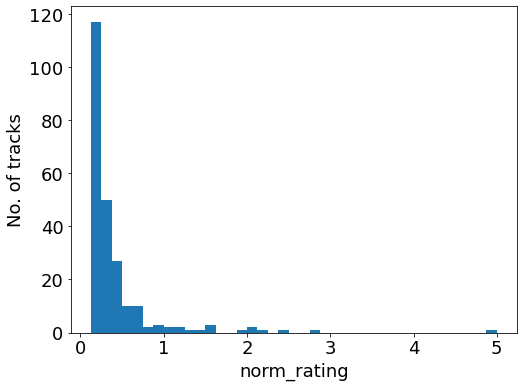
\includegraphics[width= 1\linewidth]{./images/min_max_distribution.png}
            \vspace*{-5mm}
            \caption{Min-Max Normalization}
            \label{fig:min_max_normalization}
            \vspace*{2mm}
        \end{subfigure}
        \begin{subfigure}{.48\textwidth}
            \centering
            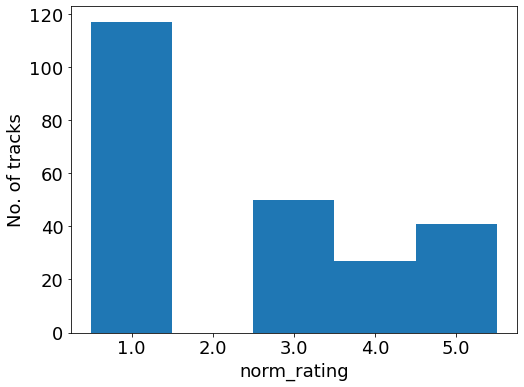
\includegraphics[width= 1\linewidth]{./images/percentile_distribution.png}
            \vspace*{-5mm}
            \caption{Percentile Normalization}
            \label{fig:percentile_normalization}
        \end{subfigure}
    \caption{Distribution of normalized ratings within one user in MuTube from different normalization strategies}
    \label{fig:Normalize_strategy_result}
    \end{center}
\end{figure}
% ----- Figure ------

\paragraph{}
Aside from distribution of normalized ratings, we use SVD model and our proposed framework to compare the results of individual recommendation from two normalization strategies and evaluate the effectiveness, the results are shown as Table.~\ref{tab:Normalization_strategy_SVD_MuTube} and Table.~\ref{tab:Normalization_strategy_proposed_MuTube}. If the items with top ``10" highest predicted ratings cannot cause user's interest, users are very likely to ignore rest of items behind the recommendation. Hence, the number of items in the recommendation list for each user is set to ``10" here. From Table.~\ref{tab:Normalization_strategy_SVD_MuTube} and Table.~\ref{tab:Normalization_strategy_proposed_MuTube}, it is evident that percentile normalization achieves better accuracy and also performs better in aspects of coverage and novelty. As a consequence, percentile normalization will be utilized to measure users' implicit feedback in the rest parts of this research.

% ----- Table ------ %
\begin{table}[!hbtp]
    \centering
    \caption{Comparison of normalization strategies from using SVD on MuTube dataset}
    \begin{tabular}{| l || c c c || c c|}
    \hline
    & \textbf{Precision} & \textbf{Recall} & \textbf{F1 Score} & \textbf{HitCov} & \textbf{HitNov}\\
    \hline
    Min-Max &  11.0\% & 1.89\% & 0.032 & 2.11\% & 7.0\% \\ 
    Percentile & \textbf{15.8\%} & \textbf{3.38\%} & \textbf{0.056} & \textbf{2.83}\% & \textbf{8.8\%} \\
    \hline
    \end{tabular}
    \label{tab:Normalization_strategy_SVD_MuTube}
\end{table}

\begin{table}[!hbtp]
    \centering
    \caption{Comparison of normalization strategies from using proposed framework on MuTube dataset}
    \begin{tabular}{| l || c c c || c c|}
    \hline
    & \textbf{Precision} & \textbf{Recall} & \textbf{F1 Score} & \textbf{HitCov} & \textbf{HitNov}\\
    \hline
    Min-Max &  48.8\% & 16.13\% & 0.242 & 10.84\% & 35.6\% \\ 
    Percentile & \textbf{49.2\%} & \textbf{16.22\%} & \textbf{0.244} & \textbf{10.94}\% & \textbf{36.0\%} \\
    \hline
    \end{tabular}
    \label{tab:Normalization_strategy_proposed_MuTube}
\end{table}
% ----- Table ----- %

\section{Evaluation of Proposed Framework}
The effectiveness of the proposed framework will be evaluated and compared with other existing methods in this section. The detailed description of existing methods is depicted as follows: 
\begin{itemize}
    \item \textbf{SVD}: We use the famous SVD method to shrink space dimensions of rating matrix, and then predict the ratings of unseen items for each users according to their behavioural data. 
    \item \textbf{Extended-SVD}: As mentioned in \cite{osmanli2011using}, tagging information is combined into the original user-item matrix. Namely, the rating matrix is augmented with user-tag pair horizontally before conducting SVD.
    \item \textbf{Filtering}: Rating data is utilized to calculate user similarity, and then filter out irrelevant users and their behavioural data before conducting SVD, which reduces the sparsity level and ``noise data" in the matrix.
\end{itemize}

\subsection{Accuracy comparison on multimedia datasets}
\paragraph{}
Table.~\ref{tab:ML_acc} represents the accuracy of different recommendation approaches for Movielens dataset while the length of recommendation list for each user is ``5", ``10", and ``20" individually. From Table.~\ref{tab:ML_acc}, we can find that the ESVD approach indeed improves the accuracy of SVD, which proves that applying tagging information to rating data can provide recommendations with higher quality. Next, it is evident that Filtering and the proposed framework outperform the other two approaches in most cases. Since the performance of Filtering and proposed framework are almost the same, we will perform more experiments for analysis and discuss which approach can provide recommendations with higher quality for users in later parts of this chapter.

% Again, we think the performance of an recommendation system is more important while the length of recommendation list is smaller; once the ``5" most-recommended items cannot capture the user's attention, the user will care about neither the top-10 recommendation list nor the top-20 recommendation list.
% --- Table  Movielens---- %
\begin{table}[!htb]
    \centering
    \caption{Recommendation accuracy of proposed framework compared to existing methods on Movielens}
    \begin{tabular}{|l || c c c c|}
    \hline
         & \multicolumn{4}{c|}{Top-5 Recommendation} \\
    \cline{2-5}
         &  \textbf{Precision} & \textbf{Recall} & \textbf{F1 Score} & \textbf{nDCG} \\
    \hline
    SVD     & 57.2\% & 3.04\% & 0.057 & 0.445 \\
    Extended-SVD & 61.6\% & 2.73\% & 0.052 & 0.518\\
    Filtering & \textbf{65.6\%} & \textbf{3.04\%} & \textbf{0.058} & \textbf{0.58}\\
    \textbf{Proposed}  & 65.1\% & \textbf{3.04\%} & \textbf{0.058} & 0.564 \\
    \hline
    \end{tabular}
    \bigskip
    
    \begin{tabular}{|l || c c c c|}
    \hline
         & \multicolumn{4}{c|}{Top-10 Recommendation} \\
    \cline{2-5}
         &  \textbf{Precision} & \textbf{Recall} & \textbf{F1 Score} & \textbf{nDCG} \\
    \hline
    SVD     & 52.2\% & 5.07\% & 0.092 & 0.452 \\
    Extended-SVD & 56.9\% & 4.89\% & 0.090 & 0.484\\
    Filtering & \textbf{60.7\%} & \textbf{5.34\%} & \textbf{0.098} & \textbf{0.553}\\
    \textbf{Proposed}  & 58.3\% & 5.12\% & 0.094 & 0.539 \\
    \hline
    \end{tabular}
    \bigskip
    
    \begin{tabular}{|l || c c c c|}
    \hline
         & \multicolumn{4}{c|}{Top-20 Recommendation} \\
    \cline{2-5}
         &  \textbf{Precision} & \textbf{Recall} & \textbf{F1 Score} & \textbf{nDCG} \\
    \hline
    SVD     & 43.2\% & 7.86\% & 0.133 & 0.427 \\
    Extended-SVD & 51.8\% & 8.29\% & 0.143 & 0.462\\
    Filtering & \textbf{54.1}\% & \textbf{8.93}\% & \textbf{0.153} & \textbf{0.526}\\
    \textbf{Proposed}  & 51.2\% & 8.49\% & 0.146 & 0.484 \\
    \hline
    \end{tabular}
    \label{tab:ML_acc}
\end{table}

\paragraph{}
Aside from Movielens, we also analyze the accuracy comparison of different recommendation approaches on MuTube dataset, the related result is shown in Table.~\ref{tab:MuTube_acc}. While our proposed framework has similar performance in aspects of accuracy compared to the Filtering approach on Movielens, it achieves better performance than all the other three approaches in all cases on MuTube dataset. We think there are two main differences between Movielens and MuTube such that the proposed framework dominates the recommendation quality on the latter dataset: sparsity and the number of tags. The recommendation quality of SVD is highly dependent on the sparsity of the user-item matrix, it thus becomes ineffective while the problem of data sparsity occurred. The sparsity of each dataset has been shown in Table.~\ref{tab:datasets}; we can find that the sparsity of MuTube is larger than which of Movielens, and this makes the other SVD-based approaches can only get poor performance on MuTube. Next, the number of tags in MuTube is way more than which in Movielens; our proposed framework generates recommendations for users relying on their tag preferences, which means that with more tagging information available, our proposed framework can acquire more information and become more effective. According to the two reasons mentioned above, our approach made a significant improvement in accuracy for MuTube.
% ----- Table MuTube ------ %
\begin{table}[!htb]
    \centering
    \caption{Recommendation accuracy of proposed framework compared to existing methods on MuTube}
    \begin{tabular}{|l || c c c c|}
    \hline
         & \multicolumn{4}{c|}{Top-5 Recommendation} \\
    \cline{2-5}
         &  \textbf{Precision} & \textbf{Recall} & \textbf{F1 Score} & \textbf{nDCG} \\
    \hline
    SVD     & 14.4\% & 1.72\% & 0.030 & 0.086 \\
    Extended-SVD & 16.8\% & 2.11\% & 0.037 & 0.074\\
    Filtering & 21.2\% & 2.28\% & 0.041 & 0.135\\
    \textbf{Proposed}  & \textbf{57.2\%} & \textbf{10.2\%} & \textbf{0.172} & \textbf{0.458} \\
    \hline
    \end{tabular}
    \bigskip
    
    
    \begin{tabular}{|l || c c c c|}
    \hline
         & \multicolumn{4}{c|}{Top-10 Recommendation} \\
    \cline{2-5}
         &  \textbf{Precision} & \textbf{Recall} & \textbf{F1 Score} & \textbf{nDCG} \\
    \hline
    SVD     & 13.5\% & 2.33\% & 0.039 & 0.077 \\
    Extended-SVD & 14.5\% & 2.69\% & 0.045 & 0.082\\
    Filtering & 18.0\% & 3.66\% & 0.061 & 0.124\\
    \textbf{Proposed}  & \textbf{49.2\%} & \textbf{16.2\%} & \textbf{0.244} & \textbf{0.427} \\
    \hline
    \end{tabular}
    \bigskip
    
    \begin{tabular}{|l || c c c c|}
    \hline
         & \multicolumn{4}{c|}{Top-20 Recommendation} \\
    \cline{2-5}
         &  \textbf{Precision} & \textbf{Recall} & \textbf{F1 Score} & \textbf{nDCG} \\
    \hline
    SVD     & 12.45\% & 4.47\% & 0.065 & 0.076 \\
    Extended-SVD & 14.55\% & 5.57\% & 0.080 & 0.083\\
    Filtering & 17.9\% & 7.19\% & 0.102 & 0.118\\
    \textbf{Proposed}  & \textbf{35.0\%} & \textbf{20.6\%} & \textbf{0.259} & \textbf{0.387} \\
    \hline
    \end{tabular}
    \label{tab:MuTube_acc}
\end{table}

\clearpage
\subsection{Analysis of diversity and novelty}
\paragraph{}
Besides the accuracy, the coverage and novelty of recommendation lists are also vital to further measure the quality of recommendations. The comparison result on both datasets are detailed in Table.~\ref{tab:ML_cov&nov} and Table.~\ref{tab:MuTube_cov&nov}. As can be seen from Table.~\ref{tab:ML_cov&nov} and Table.~\ref{tab:MuTube_cov&nov}, the Filtering approach and the proposed framework become the two best approaches in respect of diversity and novelty. For Movielens dataset, the accuracy of the Filtering approach is the best compared to other methods, which makes Filtering approach achieve better performance on $HitCov$ and $HitNov$ since both metrics consider precision of recommendations implicitly; on the other hand, our method performs slightly better than Filtering in terms of $Cov$ and $Nov$. Since both recommendation approaches has their pros and cons, it becomes a problem to decide which approach is better overall. As a result, we analyze the performance of four approaches for MuTube dataset, which is shown as Table.~\ref{tab:MuTube_cov&nov}, and it is evident that our proposed framework outperforms the other approaches in all cases for MuTube, including Filtering approach.

% ----- Table diversity and novelty ------
\begin{table}[!htp]
    \centering
    \caption{Coverage and novelty of proposed framework compared to existing methods on Movielens}
    \begin{tabular}{|l ||c c| c c |}
    \hline
        & \multicolumn{4}{c|}{Top-5 Recommendation} \\
    \cline{2-5}
        &  \textbf{COV} & \textbf{HitCov} & \textbf{NOV} & \textbf{HitNov} \\
    \hline
     SVD               &  0.39\%  & 0.38\% & 0.677 & 0.365 \\
     Extended-SVD      &  0.39\%  & 0.37\% & 0.645  & 0.399  \\ 
     Filtering         &  1.93\%  & \textbf{1.72}\% & 0.679 & \textbf{0.457}   \\
     \textbf{Proposed} &  \textbf{2.73\%} & 1.38\% & \textbf{0.682} & 0.438  \\
     \hline
    \end{tabular}
    \bigskip
    
    \begin{tabular}{|l ||c c| c c |}
    \hline
        & \multicolumn{4}{c|}{Top-10 Recommendation} \\
    \cline{2-5}
        &  \textbf{COV} & \textbf{HitCov} & \textbf{NOV} & \textbf{HitNov} \\
    \hline
     SVD               &  0.61\%  & 0.60\% & 0.688 & 0.351 \\
     Extended-SVD      &  0.65\%  & 0.64\% & 0.666 & 0.378 \\ 
     Filtering         &  2.74\%  & \textbf{2.50}\% & 0.699 & \textbf{0.433}  \\
     \textbf{Proposed} &  \textbf{4.42\%} & 2.04\% & \textbf{0.704} & 0.404  \\
     \hline
    \end{tabular}
    \bigskip
    
    \begin{tabular}{|l ||c c| c c |}
    \hline
        & \multicolumn{4}{c|}{Top-20 Recommendation} \\
    \cline{2-5}
        &  \textbf{COV} & \textbf{HitCov} & \textbf{NOV} & \textbf{HitNov} \\
    \hline
     SVD               &  0.99\%  & 0.98\% & 0.715 & 0.318 \\
     Extended-SVD      &  1.06\%  & 1.05\% & 0.687 & 0.355 \\ 
     Filtering         &  4.49\%  & \textbf{3.83}\% & 0.722 & \textbf{0.397}  \\
     \textbf{Proposed} &  \textbf{6.85\%} & 3.09\% & \textbf{0.725} & 0.364 \\
     \hline
    \end{tabular}
    \label{tab:ML_cov&nov}
\end{table}

\begin{table}[!htb]
    \centering
    \caption{Coverage and novelty of proposed framework compared to existing methods on MuTube}
    \begin{tabular}{|l ||c c| c c |}
    \hline
        & \multicolumn{4}{c|}{Top-5 Recommendation} \\
    \cline{2-5}
        &  \textbf{COV} & \textbf{HitCov} & \textbf{NOV} & \textbf{HitNov} \\
    \hline
     SVD               &  3.07\%  & 1.25\% & 0.657 & 0.078 \\
     Extended-SVD      &  3.31\%  & 1.53\% & 0.615 & 0.087 \\ 
     Filtering         &  7.29\%  & 2.21\% & 0.686 & 0.129  \\
     \textbf{Proposed} &  \textbf{10.17\%} & \textbf{6.28\%} & \textbf{0.761} & \textbf{0.420}  \\
     \hline
    \end{tabular}
    \bigskip
    
    \begin{tabular}{|l ||c c| c c |}
    \hline
        & \multicolumn{4}{c|}{Top-10 Recommendation} \\
    \cline{2-5}
        &  \textbf{COV} & \textbf{HitCov} & \textbf{NOV} & \textbf{HitNov} \\
    \hline
     SVD               &  5.76\%  & 2.69\% & 0.669 & 0.086 \\
     Extended-SVD      &  5.76\%  & 2.88\% & 0.634 & 0.088 \\ 
     Filtering         &  12.28\%  & 3.65\% & 0.705 & 0.112  \\
     \textbf{Proposed} &  \textbf{18.18\%} & \textbf{10.94\%} & \textbf{0.760} & \textbf{0.360}  \\
     \hline
    \end{tabular}
    \bigskip
    
    \begin{tabular}{|l ||c c| c c |}
    \hline
        & \multicolumn{4}{c|}{Top-20 Recommendation} \\
    \cline{2-5}
        &  \textbf{COV} & \textbf{HitCov} & \textbf{NOV} & \textbf{HitNov} \\
    \hline
     SVD               &  11.32\%  & 5.42\% & 0.697 & 0.093 \\
     Extended-SVD      &  11.22\%  & 5.23\% & 0.665 & 0.084 \\ 
     Filtering         &  17.99\%  & 7.29\% & 0.723 & 0.116  \\
     \textbf{Proposed} &  \textbf{28.87\%} & \textbf{15.16\%} & \textbf{0.758} & \textbf{0.252}  \\
     \hline
    \end{tabular}
    \label{tab:MuTube_cov&nov}
\end{table}

\newpage
\clearpage
\subsection{Response time analysis}
\paragraph{}
The response time for a recommendation approach also plays a vital role in evaluating the performance of a recommender system, a good recommender system not only means that it can meet users' preferences but also can generate recommendations without too much time for computation. If the time required for making recommendations is too long, some users may become impatient and thus lose interest. Hence, we would like to analyze the response time of each recommendation approach mentioned above and find the most suitable recommendation approach for each media considering the trade-off between recommendation quality and response time. Table.~\ref{tab:response_time} presents the average response time required for the compared recommendation approaches to generate recommendations for a single user on two datasets. We find that the proposed framework has the shortest response time, which indicates that it can generate recommendations without taking too much time; while Filtering is the most time-consuming approach since it must filter out irrelevant information before making recommendations. Although the Filtering method can generate the best recommendations for Movielens in the aspect of accuracy, the response time of our proposed framework is dominant no matter which dataset is used. Here, we think the scale of the dataset affects the improvement of the proposed framework in the aspect of response time since the scale of Movielens is way larger than which of MuTube. The improvement in response time of our proposed framework for Movielens (13 times faster) is more obvious than which for MuTube (4.8 times faster). We can infer that our proposed framework has more advantages in response time while the scale of the dataset used is larger.

\begin{table}[!htb]
    \centering
    \caption{Response time required to generate recommendation list for a single user}
    \begin{tabular}{|l||c c|}
    \hline
         & MovieLens & MuTube \\
    \hline
    SVD  &  0.024s     & 0.0023s\\
    ESVD &  0.024s     & 0.0021s\\ 
    Filtering & 0.121s & 0.0048s\\ 
    Proposed & \textbf{0.009s}  & \textbf{0.0010s}\\ 
    \hline
    \end{tabular}
    \label{tab:response_time}
\end{table}

\subsection{Overall Analysis}
\paragraph{}
Table.~\ref{tab:overall_eva} presents the overall evaluation of proposed framework and the other existing approaches for MovieLens and MuTube individually. The values in the table are the average of Top-5, Top-10, and Top-20 over MovieLens and MuTube dataset. Although the Filtering approach performs slightly better than our proposed framework in terms of accuracy for Movielens dataset, it will become extremely time-consuming for datasets with an immense amount of information as mentioned in Table.~\ref{tab:response_time}. As for our proposed framework, it is evident that our approach can deal with large-scale datasets without taking too much time; furthermore, our method also performs well in terms of accuracy, diversity, and novelty. In summary, we can conclude that our proposed framework is an effective methodology that not only generates recommendations with high quality but considers and finds the trade-off between accuracy and response time.

\begin{table}[!htb]
    \centering
    \caption{Overall Evaluation on two datasets}
    \begin{tabular}{|l||c c c c| c c| c c |}
    \hline
        & \multicolumn{8}{c|}{MovieLens} \\
    \cline{2-9}
        & Prec. & Rec. & F1 & nDCG & Cov & HitCOV & Nov & HitNOV  \\
    \hline
        SVD &  51.08\% & 5.50\% & 0.097 & 0.451 & 0.66\% & 0.65\% & 0.693 & 0.345 \\
        ESVD & 56.79\% & 5.31\% & 0.095 & 0.499 & 0.70\% & 0.69\% & 0.665 & 0.377 \\
        Filtering & \textbf{60.17\%} & \textbf{5.78\%} & \textbf{0.103} & \textbf{0.559} & 3.05\% & \textbf{2.70\%} & 0.699 & \textbf{0.428} \\
        Proposed &  58.15\% & 5.55 & 0.099 & 0.538 & \textbf{4.66\%} & 2.17\% & \textbf{0.703} & 0.402 \\
    \hline
    \end{tabular}
    \bigskip
    
    \begin{tabular}{|l||c c c c| c c| c c |}
    \hline
        & \multicolumn{8}{c|}{MuTube} \\
    \cline{2-9}
        & Prec. & Rec. & F1 & nDCG & Cov & HitCOV & Nov & HitNOV  \\
    \hline
        SVD &  14.97\% & 3.70\% & 0.057 & 0.089 & 6.71\% & 3.12\% & 0.67 & 0.0859 \\
        ESVD & 15.96\% & 4.20\% & 0.064 & 0.076 & 6.76\% & 3.21\% & 0.64 & 0.0863 \\
        Filtering & 19.03\% & 4.38\% & 0.068 & 0.126 & 12.51\% & 4.38\% & 0.70 & 0.1193 \\
        Proposed &  \textbf{47.07\%} & \textbf{15.63\%} & \textbf{0.224} & \textbf{0.424} & \textbf{19.07\%} & \textbf{10.79\%} & \textbf{0.76} & \textbf{0.3440} \\
    \hline
    \end{tabular}
    \label{tab:overall_eva}
\end{table}

%*-------------------Performance Evaluation--------------------------
%*--------------------------Conclusion-------------------------------
\chapter{Conclusion}
\paragraph{}
In this work, we propose a framework that uses tags provided in the dataset to find users' tag preferences and make recommendations based on tag preference and the item-tag pair. First, we show how to measure users' implicit feedback while explicit feedback is not available in the dataset, we choose percentile normalization as the normalization strategy to transform the listening counts into normalized ratings. Next, tagging information including tag relevance and tag preference is used to find the Top-N most suitable items for users. Finally, a recommendation list is generated for each user in the dataset. We demonstrate the proposed framework on two real-world datasets: the famous MovieLens and the MuTube dataset. Experimental result shows that our proposed framework not only successfully finds the trade-off between recommendation quality and response time but performs well in terms of accuracy for both datasets.
%---
\paragraph{}
We only use historical data in this work, which means that the performance of each recommendation approach is evaluated based on offline evaluation. We cannot actually measure users' satisfaction by using offline evaluation only. To evaluate the effectiveness of our proposed framework in real-world systems and see if items recommended by our method can indeed capture users' interests, we would like to create an online system that can help us to know users' feedback on recommendation lists provided. Also, our proposed framework considers only tagging information in this work. We think the other factors such as genres can also be combined with our framework to further optimize the recommendations in the future.
%*--------------------------Conclusion-------------------------------
\newpage
\addcontentsline{toc}{chapter}{Bibliography}
\bibliographystyle{IEEEtran}
\bibliography{references}

\end{document}

